\chapter{LadarSIM Modification}

\section{LadarSIM Background}

LadarSIM is a robust parameterized tool for simulating lidar systems, which has been
developed at Utah State University's Center for Advanced Imaging Ladar (CAIL) since 2003
\cite{budgeLeishman,neilsenBudge}. LadarSIM was originally developed to simulated pulsed 
time-of-flight lidar systems and has the flexibility to simulate
a wide range of these systems by simulating parameterized lidar transceiver, focal plane 
arrays, and pointing/scanning systems, as well as the interaction of the lidar with a 
simulated 3D scene. 

The main LadarSIM GUI is shown in figure \ref{fig:LadarSIM}. The GUI is split into three basic 
sections. In brown colored section in the center controls basic simulation parameters, such as
scene selection, simulation fidelity, and what files the simulation will save. 

The green section on the left side of the GUI is the geometry simulation. This section simulates
the scenario from a strictly geometric stand point. This simulation produces a point cloud using 
the scanner parameters, sensor flight path, and scene. The geometric simulation runs independently
of the type of lidar to be simulated. The geometric measurements generated by the geometry simulation
are used when LadarSIM simulates the actual performance of the specified lidar system. 

The blue section on the right side of the GUI is the radiometric simulation. Again this cannot be run
until after a geometric simulation of the scenario has been run. This side of the of the GUI can be used
to simulate the performance of a particular lidar configuration. Parameters relating to the optical efficiency, 
transmitted beam, receiver, and range processing can be customized. The purpose of separating the geometric 
and radiometric simulations is that the output of a single geometric simulation can be used to evaluate the 
performance of different lidar configurations. 

\begin{figure}[!htb]
	\centering
	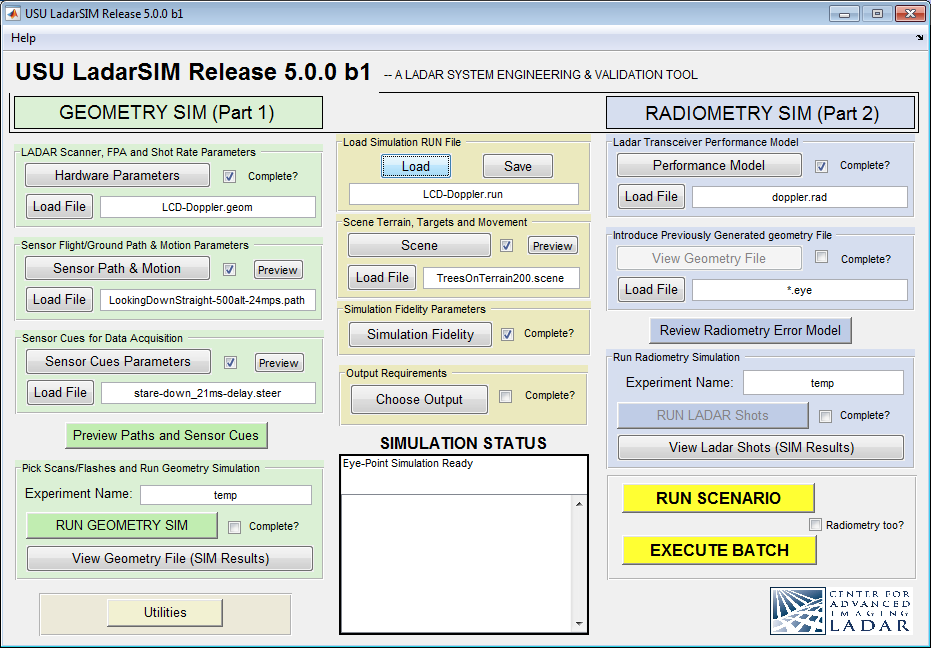
\includegraphics[width=.8\columnwidth]{figs/LadarSIM}
	\vspace{1em}
	\caption{Main GUI for running LadarSIM.}
	\label{fig:LadarSIM}
\end{figure}
